\documentclass[11pt,openright,twoside,french]{book}

\input philippe2013
\input philippe2013_activites

\pagestyle{empty}

\begin{document}

\TitreExo{A}{Translations \\ Relation de Chasles}

\exo 

\begin{minipage}{0.7\linewidth}
	Sur la figure ci-contre sont représentés six hexagones réguliers.
	\begin{enumerate}
		\item Déterminer le point $M_1$ tel que $\vect{AM_1} = \vect{CD}$.
		\item Déterminer les points $M_2$, $M_3$ et $M_4$ tels que
		\[\vect{AM_2} = \vect{FD} \qq \vect{CM_3} = \vect{DB} \qetq \vect{FM_4} = \vect{EC}.\]
		\item Déterminer les points $N_1$, $N_2$ et $N_3$ tels que :
		\[\vect{AN_1} = \vect{AB} + \vect{AC} \qq \vect{AN_2} = \vect{ED} + \vect{CH} \qetq \vect{FN_3} = \vect{AC} + \vect{FB}.\]
		\item Déterminer les points $P_1$, $P_2$ et $P_3$ tels que :
		\[\vect{AP_1} = \vect{AB} + \vect{AC} + \vect{BF} \qq \vect{JP_2} = \vect{BE} + \vect{CD} + \vect{BH} \qetq \vect{KP_3} = \vect{DA} + \vect{GB} + \vect{BA}.\]
	\end{enumerate}
\end{minipage}
\begin{minipage}{0.3\linewidth}
\begin{center}
	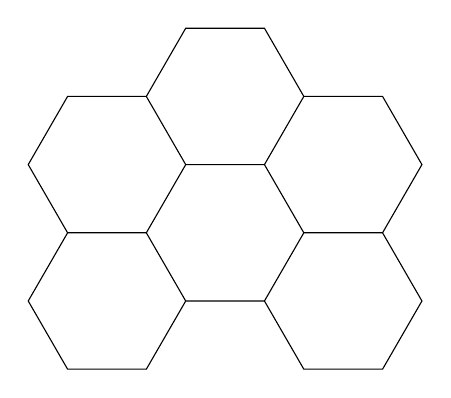
\begin{tikzpicture}
		\draw (0,0) -- ++(1,0) -- ++(60:1) -- ++(1,0) -- ++(-60:1) -- ++ (1,0) -- ++(-60:1) -- ++(-120:1) -- ++(-60:1) -- ++(-120:1) -- ++(-1,0) -- ++(120:1) -- ++(-1,0) -- ++(-120:1) -- ++(-1,0) -- ++(120:1) -- ++(60:1) -- ++(120:1) -- cycle;
		\draw (0,-1.732) -- ++(1,0) -- ++ (60:1) -- ++(1,0) -- ++(-60:1) -- ++ (1,0);
		\draw (1,-1.732) -- ++(-60:1);\draw (3,-1.732) -- ++(-120:1);
		\draw (1,0) -- ++(-60:1);\draw (3,0) -- ++(-120:1);
	\end{tikzpicture}
\end{center}
\end{minipage}
\[*\]

\exo Les points $A$, $B$, $C$ et $D$ étant quelconques, démontrer l'égalité (sans faire de figure !) :
\[3\vect{DA} - \vect{DB} - 2\vect{DC} = 3\vect{BA} - 2\vect{BC}.\]
\[*\]

\exo Soit $ABCD$ un parallélogramme de centre $O$.\par
On considère les points $E$ et $F$ tels que :
\begin{itemize}
	\item $\vect{DF} = \vect{AO}$
	\item $\vect{AE} = 2\vect{AB} + 2\vect{AD}$
\end{itemize}

\begin{enumerate}
	\item Faire une figure.
	\item Exprimer le vecteur $\vect{AE}$ en fonction du vecteur $\vect{AC}$.
	\item Démontrer que les vecteurs $\vect{AE}$ et $\vect{DF}$ sont colinéaires.
	\item Déterminer la nature du quadrilatère $AEFD$.
\end{enumerate}



\end{document} 